\chapter{Deployment View and Transfer Sequence}
\label{chap:appendixB}

This appendix gives two diagrams that complement the architectural narrative of Chapter~\ref{chap:methodology}. The first is the deployed component view of the system; the second is the call sequence of a partner-mediated transfer from the operator's tap to the server-side acknowledgement.

\section{Deployed Component View}
\label{sec:appB-components}
\begin{figure}[h]
  \centering
  \begin{tikzpicture}[
    node distance=8mm and 10mm,
    box/.style={draw, rounded corners=2pt, minimum width=32mm, minimum height=8mm,
                font=\small, align=center, fill=blue!5},
    server/.style={draw, rounded corners=2pt, minimum width=32mm, minimum height=8mm,
                   font=\small, align=center, fill=gray!10},
    arr/.style={->, thick}
  ]
    \node[box] (ui)      {Flutter UI\\(Widgets, Theme)};
    \node[box, below=of ui] (bloc)    {BLoC / Cubit};
    \node[box, below=of bloc] (uc)    {Use cases\\(domain layer)};
    \node[box, below=of uc]   (repo)  {Repositories};
    \node[box, below=of repo] (ds)    {Supabase data sources\\(typed RPC, REST)};
    \node[server, below=of ds] (sb)   {Supabase\\(PostgreSQL\,16, RLS,\\PL/pgSQL, Realtime)};

    \draw[arr] (ui)   -- (bloc);
    \draw[arr] (bloc) -- (uc);
    \draw[arr] (uc)   -- (repo);
    \draw[arr] (repo) -- (ds);
    \draw[arr] (ds)   -- (sb);
    \draw[arr, dashed] (sb.west) to[bend left=45] node[font=\scriptsize, midway, left]{Realtime\\(logical replication)} (bloc.west);
  \end{tikzpicture}
  \caption{Deployed component view of \emph{Ethnocount}. Solid arrows are the write-path call flow; the dashed arrow is the Realtime change feed that refreshes the BLoCs after remote writes.}
  \label{fig:components}
\end{figure}

\section{Partner-Mediated Transfer Sequence}
\label{sec:appB-sequence}
\begin{figure}[h]
  \centering
  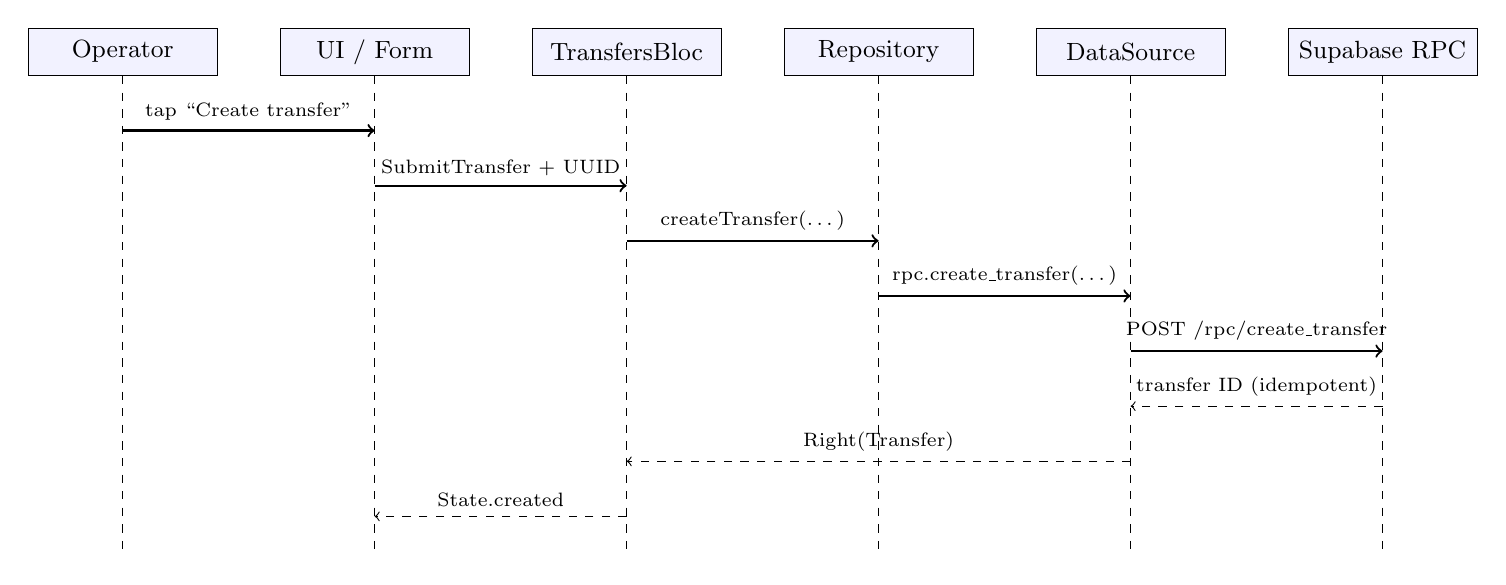
\begin{tikzpicture}[
    actor/.style={draw, fill=blue!5, font=\small, minimum width=24mm, minimum height=6mm},
    msg/.style={->, thick, font=\scriptsize},
    return/.style={->, dashed, font=\scriptsize}
  ]
    \node[actor] (u)    at (0,0)  {Operator};
    \node[actor] (ui)   at (3.2,0)  {UI / Form};
    \node[actor] (b)    at (6.4,0)  {TransfersBloc};
    \node[actor] (r)    at (9.6,0)  {Repository};
    \node[actor] (ds)   at (12.8,0) {DataSource};
    \node[actor] (sb)   at (16,0)   {Supabase RPC};

    \foreach \n in {u,ui,b,r,ds,sb} \draw[dashed] (\n) -- ++(0,-6.4);

    \draw[msg]   (0,-1)   -- node[above]{tap ``Create transfer''} (3.2,-1);
    \draw[msg]   (3.2,-1.7) -- node[above]{SubmitTransfer + UUID} (6.4,-1.7);
    \draw[msg]   (6.4,-2.4) -- node[above]{createTransfer(\ldots)} (9.6,-2.4);
    \draw[msg]   (9.6,-3.1) -- node[above]{rpc.create\_transfer(\ldots)} (12.8,-3.1);
    \draw[msg]   (12.8,-3.8) -- node[above]{POST /rpc/create\_transfer} (16,-3.8);
    \draw[return] (16,-4.5) -- node[above]{transfer ID (idempotent)} (12.8,-4.5);
    \draw[return] (12.8,-5.2) -- node[above]{Right(Transfer)} (6.4,-5.2);
    \draw[return] (6.4,-5.9) -- node[above]{State.created} (3.2,-5.9);
  \end{tikzpicture}
  \caption{Sequence of a partner-mediated transfer from the operator's tap to the server-side acknowledgement. The idempotency key (a UUID generated client-side in the form's initialiser) travels with the request and is stored against a UNIQUE partial index on the server, so a duplicate request returns the original transfer ID rather than creating a second row.}
  \label{fig:sequence}
\end{figure}
